

%%%%%%%%%%%%%%%%%%%%%%%%%%%%%%%%%%%%%%%%
\subsection{Setup and Proof of \cref{main_result}}
\label{KeyTools}

1. Imagine trying to solve a poblem\\
2. vertex lives in possibly many bags, motivates home\\
3. label in home log n
4. indentifying home bag log n (or testing if two vertices in the same bag another log n bits)
5. already at 2 log n and it does not solve a problem 
6. stop clever person here, although the internal lable in the and the idetification of its bag can be reduces to log n ... it does not solve adjenecny proble (stupid n log n does)
7. to be able to do adjecncy testing (more effeciently) we introduce mixed labelling schmem -- has somehow two properties
- it can test adjecency
- it encosed this path ... this would work except that this path may be of lenght log n. 
- works but the solution uses log n + h*w(1) bits

- to handle that we need tree decompositions of short hight

\david{Can the text from the start of 1.2 to here be removed or moved elsewhere?}

We now introduce one result from the literature, \cref{gmpst}, and three technical results, \cref{PlainRealMainTechnical,HandleApexvertices,gk_labelling}, which together prove \cref{main_result}. First we need several definitions.

In this paper, all graphs are finite, simple, and undirected.  For a graph $G$, \defin{$V(G)$} denotes the vertex-set of $G$, \defin{$E(G)$} denotes the edge-set of $G$.  A \defin{clique} in a graph is a non-empty set of pairwise adjacent vertices.   Let $G$ be a graph and $X\subseteq V(G)$. By $G[X]$ we denote the subgraph of $G$ induced on $X$. For other standard graph theory terms, we refer the reader to the textbook by \citet{diestel:graph}.

A \defin{graph class} is a set of graphs closed under isomorphism. A graph class  $\calG$ is \defin{hereditary} if for every $G$ in $\calG$ every induced subgraph of $G$ is also in $\calG$. A  graph class $\calG$ is \defin{monotone} if for every $G\in\calG$, every subgraph of $G$ is in $\calG$.
A  graph class $\calG$ is \defin{minor-closed} if for every $G\in\calG$, every minor of $G$ is in $\calG$. A graph class $\calG$ is \defin{proper} if some graph is not in $\calG$.  A \defin{disjoint union} of two graphs $G$ and $H$ is a graph obtained from two vertex-disjoint copies of $G$ and $H$ with no edge in between. A class of graphs $\calC$ is \defin{closed under taking disjoint union} if for all $G,H$ in $\calC$, the disjoint union of $G$ and $H$ is also in $\calC$.

%Our main technical result, from which \cref{main_result} follows, is stated in terms of tree-decompositions.  We first introduce the necessary notation before giving an overview of the proof. 
A \defin{tree-decomposition} of a graph $G$ is a pair $(T,(B_x \mid x \in V(T)))$,
where $T$ is a tree and $B_x \subseteq V(G)$ for every $x \in V(T)$, with the
following properties:
\begin{enumerate*}[label=(\alph*)]
  \item for each vertex $u$ in $G$, the subgraph of $T$ induced by $\{x \in V(T) \mid u \in B_x\}$ is non-empty and connected; and
  \item for each edge $uv$ in $G$, there exists $x\in V(T)$ such that $u,v\in B_x$.
\end{enumerate*}
We call the sets $B_x$ the \defin{bags} of the tree-decomposition and the sets $B_x\cap B_y$ for all distinct $x,y\in V(T)$, the \defin{adhesions} of the tree-decomposition.
The \defin{width} of a tree-decomposition is the maximum size of a bag minus one.
The \defin{adhesion-width} of a tree-decomposition is the maximum size of an adhesion.
(In the literature, adhesions are usually defined only for pairs $x,y \in V(T)$ with $xy \in E(T)$; we remark that adhesion-width is the same under the two definitions.)\
\pat{There was an old discussion about this. We only need adhesions to be defined for neighbouring bags.} \david{Then I suggest we define adhesions only for $xy\in E(T)$, which is standard.} For a tree-decomposition $(T,(B_x \mid x\in V(T)))$ of a graph $G$, for each  $x\in V(T)$, the \defin{torso} of $x$, denoted by \defin{$\torso{G}{B_x}$}, is the graph with the vertex-set $B_x$ in which two distinct vertices $u$ and $v$ are adjacent if $uv \in E(G)$, or there exists $y \in N_T(x)$  such that $u,v \in B_x \cap B_y$.\footnote{For a graph $G$ and a vertex $v$ of $G$, $N_G(v)$ denotes a set of neighbours of $v$ in $G$. The notation $\torso{G}{B_x}$ introduces some minor ambiguity since the definition of $\torso{G}{B_x}$ depends on $(B_y:y\in N_T(x))$, but the notation makes no reference to the tree-decomposition $(T, (B_z\mid z\in V(T))$.  When we use this notation, the tree-decomposition will always be obvious from context.} 


%Let $G$ be a graph and $\calT=(T,(B_x \mid x\in V(T)))$ be a tree-decomposition of $G$. If $T$ is a path, then $\calT$ is a \defin{path-decomposition} of $G$, simply denoted by the sequence $(W_1, W_2, \dots, W_m)$ of the bags in the order of the vertices in the underlying path.

%\david{Do we really want to define "adhesion" for any distinct $x,y \in V(T)$. It is standard to define adhesion only if $xy \in E(T)$. Of course, the adhesion-width is the same under the two definitions. } \gwen{I added a remark about this in the text. I suggest we leave it this way unless it is clear that the standard definition is enough later on.}

The \defin{strong product} of graphs~$A$ and~$B$, denoted by~${A \boxtimes B}$, is the graph with vertex-set ${V(A) \times V(B)}$, where distinct vertices ${(v,x),(w,y) \in V(A) \times V(B)}$ are adjacent if
${v=w}$ and ${xy \in E(B)}$, or
${x=y}$ and ${vw \in E(A)}$, or
${vw \in E(A)}$ and~${xy \in E(B)}$.
For an integer $k\geq 0$, let \defin{$\calR_{k}$} be the class of graphs isomorphic to a subgraph of $H\boxtimes P$ for some graph $H$ with treewidth at most $k$ and for some path $P$.
The main result of \citet{dujmovic.esperet.ea:adjacency} is a $(1+o(1))\log n$-bit adjacency labelling scheme for the class $\calR_k$, for any fixed $k$.
This immediately gives $(1+o(1))\log n$-bit adjacency labelling schemes for many classes of interest.
% For example, \citet{dujmovic.joret.ea:planar} showed that $\calR_{8}$ includes all planar graphs.  
% As mentioned in the introduction, a minor-closed class 
% admits a product structure if and only if it excludes some apex graph as a minor; see \citep{Dujmovic26,DHJLW21,DujWoo-ECM} for surveys on graph product structure theory.  
A class of graphs $\calG$ admits a \defin{product structure}, if there exists an integer $k$ such that $\calG\subseteq \calR_k$. As mentioned in the introduction, a minor-closed class admits a product structure if and only if it excludes some apex graph as a minor; see \citep{Dujmovic26,DHJLW21,DujWoo-ECM} for surveys on graph product structure theory.  

To deal with arbitrary proper minor-closed classes, a broader structure is needed, which is provided by the following variant of the Robertson--Seymour Graph Minor Structure Theorem, due to \citet{dujmovic.joret.ea:planar}. For any class $\calG$, let \defin{$\calG^{+a}$} be the class of graphs $G$ such that $G-X$ is in $\calG$ for some $X\subseteq V(G)$ with $|X|\leq a$.  It is an simple exercise to show that any $(1+o(1))\log n$-bit adjacency labelling scheme for a graph class $\calG$ implies the existence of a $(1+o(1))\log n$-bit adjacency labelling scheme for $\calR^{+a}$.  In particular, for any fixed $k,a\ge 0$, there exists a $(1+o(1))\log n$-bit adjacency labelling scheme for $\calR^{+a}_k$.

\begin{thm}[\protect Graph Minor Product Structure Theorem~\citep{dujmovic.joret.ea:planar}]
  \label{gmpst}
  For every proper minor-closed class $\calG$ there exist integers $k,a\geq 0$ such that every graph in $\calG$ has a tree-decomposition in which every torso is in $\calR_k^{+a}$.
\end{thm}

%Note that \citet{dujmovic.joret.ea:planar} employed \cref{gmpst} to reprove the result of \citet{devos2004} mentioned in the introduction, which \citet{gavoille.labourel:shorter} used to construct a ${(2+o(1))\log n}$-bit adjacency labelling scheme for any proper minor-closed class. \pat{Consider removing the previous sentence.}\vida{I think i would remove it too} \david{okay}



\pat{New text} \david{add friendly sentence ... At the heart of this paper is the question of how to construct adjacency labelling schemes for graph classes defined by a tree-decomposition (as in \cref{gmpst}). First note that ... }
\Cref{gmpst} and the adjacency labelling scheme for product structured graphs in \cite{dujmovic.esperet.ea:adjacency} imply that every $n$-vertex $H$-minor-free graph $G$ has a tree-decomposition $\calT:=(T,(B_x\mid x\in V(T))$ such that the induced subgraph $G[B_x]$ has an adjacency labelling with labels of length $(1+o(1))\log n$, for each $x\in V(T)$.  Unfortunately \david{Replace `Unfortunately' by `However'}, a vertex $v$ of $G$ can appear in $B_x$ for arbitrarily many $x\in V(T)$, but \david{and} we can only afford to assign one label of length $\log n+o(\log n)$ to $v$.  This forces us to assign one `home' $x\in V(T)$ to $v$ and assign a label $\ell(v)=\ell_x(v)$ in $G[B_x]$. \david{rewording ... 
This forces $v$ to be assigned one `home' $x\in V(T)$ and to be assigned a label $\ell(v)=\ell_x(v)$ in $G[B_x]$. }
This immediately causes a problem:  For an edge $vw$ of $G$, the home $x$ assigned to $v$ may not be the same as the home $y$ assigned to $w$.  This makes the labels $\ell_x(v)$ and $\ell_y(w)$ incompatible since they come from  different graphs $G[B_x]$ and $G[B_y]$.  
% There is no reliable way to check for a tester to check for the presence of the edge $vw$.  In particular, there is no way to distinguish between $v$ and some other vertex $v'\in B_x$ that is not adjacent to $w$.
Even worse, the naïve labelling described above does not even make it possible for an adjacency tester to determine if two vertices $v$ and $w$ have the same home, i.e., to test if $x=y$.  Thus, any labelling scheme based on the tree-decomposition $\calT$ needs to solve two problems: 
\begin{enumerate*}[label=(\roman*)]
  \item\label{test_homes} it must be possible, from the labels of $v$ and $w$ to determine if the home of $v$ and the home of $w$ are the same; and
  \item\label{hard_adjacency_test} when the home of $v$ and $w$ are not the same, it must be possible to test if $v$ and $w$ are adjacent.
\end{enumerate*}

An important contribution of the current work is to introduce a generalization of adjacency labelling, called mixed labelling, that solves \ref{test_homes} and \ref{hard_adjacency_test}. Very roughly, the label for a vertex $v$ whose home is $B_x$ consists of a prefix that describes the path $x_0,\ldots,x_p$ from the root $x_0$ of $T$ to the home node $x=x_p$ of $v$ followed by an adjacency label for $v$ in $G[B_x]$.  Each step $x_{i}x_{i+1}$ in the path is described by a label for the adhesion $B_{x_i}\cap B_{x_{i+1}}$ which forms a clique in $\torso{G}{\calT,B_{x_i}}$.  One consequence of this (if we choose the homes of vertices appropriately) is that in the situation described in the previous paragraph, the path $x_0,\ldots,x_q$ from the root of $T$ to the home $y=x_q$ of $w$ will contain the home $x=x_p$ of $v$.  Furthermore, if $x\neq y$, the label of $w$ will contain the label of a clique $K$ in $\torso{\calT,G}{B_x}$ that contains $v$.  The label of $K$ and a short \emph{local identifier} of $v$ in $K$ that gets stored in the label of $w$ then makes it possible to distinguish $v$ from other nodes in $B_x$.  
\pat{End of new text} \david{checked, it is excellent}

% \pat{Here is a place that we can add some intuition about (i)~the difficulty of the problem and (ii)~the need for clique labels.  The difficulty comes from the fact that a vertex $w$ may be adjacent to a vertex $v$ whose home node $x$ is very far from the home node $y$ of $w$.  Clique labels (and local identifiers) give a way of encoding the path from the root of $T$ to the home node of $w$ so that this path contains information about a clique in $\torso{G}{B_x}$ that contains $v$.}

% To construct adjacency labelling schemes for graph classes defined by tree-decompositions (as in \cref{gmpst}), we work in the following more general setting. 
The following definition is motivated by the discussion in the previous two paragraphs. Let $\calG$ be a class of graphs.
Let $g_i:\N\to\R^+$ for each $i\in[3]$.
The class  $\calG$ admits a \defin{weighted $(g_1,g_2,g_3)$ mixed labelling scheme} of $\calG$ if there exists a pair $(A,I)$ with
\begin{itemize}[nosep,nolistsep]
  \item $A:(\{0,1\}^*)^2\to\{0,1\}$ (the \defin{adjacency tester}); and
  \item $I:(\{0,1\}^*)^3\to\{0,1\}$ (the \defin{identity tester})
\end{itemize}
such that
for every natural $n\in\N^+$,
every $n$-vertex graph $G^+$ in $\calG$,
every spanning subgraph $G$ of $G^+$, and
every weight function $\omega:V(G)\to \R^+$,
there exists an injective function $\mu: V(G)\cup K(G^+) \to \set{0,1}^*$ and a function $\kappa:\{(K, u)\mid \textrm{$K$ clique in $G^+$}, u\in K\}\to \set{0,1}^*$
such that:
\begin{enumerate}[nosep,nolistsep,label=(\roman*)]
  \item for all $u,v\in V(G)$,
        \[
          \textrm{$A(\mu(u),\mu(v))=1$ if and only if $uv\in E(G)$;}
        \]
  \item for every clique $K$ in $G^+$, $u\in K$, $v\in V(G)$,
        \[
          \textrm{$I(\mu(K),\kappa(K, u),\mu(v))=1$ if and only if $u=v$;}
        \]
  \item for every $v\in V(G)$,
        \[
          |\mu(v)| \leq \log \omega(G) - \log\omega(v) + g_1(n);
        \]
  \item for every clique $K$ in $G^+$,
        \[
          |\mu(K)|\le \log \omega(G) - \log\min_{v\in K}(\omega(v)) + g_3(n);
        \]
  \item  for every clique $K$ in $G^+$ and $u\in K$,
        \[
          |\kappa(K, u)| \leq g_2(n).
        \]
\end{enumerate}
A pair $(\mu,\kappa)$ that satisfies the first two conditions is a \defin{mixed labelling} of $(G^+,G)$ for $(A,I)$.  A pair $(\mu,\kappa)$ that satisfies all these conditions is a \defin{weighted $(g_1,g_2,g_3)$ mixed labelling} of $(G^+,G,\omega)$ for $(A,I)$.


Here is a little intuition about these definitions. Function $g_1(n)$ measures how much the length of a vertex label exceeds the ideal value $\log \omega(G) - \log\omega(v)$ that appears in Kraft's Inequality \cite{Kraft1949}. Function $g_2(n)$ is the length of the longest local identifier. Function $g_3(n)$ measures how much the length of a clique label exceeds the Kraft-like quantity $\log\omega(G)-\log\min_{v\in K}(\omega(v))$.

The existence of a weighted $(g_1(n),\cdot,\cdot)$ mixed labelling scheme for a graph class $\calG$ immediately implies the existence of a $(\log n+g_1(n))$-bit adjacency labelling scheme for $\calG$. Thus, we are interested in the case where $g_1(n)\in o(\log n)$. We say that a graph class $\calG$ admits an \defin{efficient} weighted mixed labelling scheme if $\calG$ admits a weighted $(g_1,g_2,g_3)$ mixed labelling scheme with $g_i(n)\in o(\log n)$ for each $i\in [3]$. So a graph class admitting an efficient mixed weighted labelling scheme admits a $(1+o(1))\log n$-bit adjacency labelling scheme.

Our first tool handles product structured graphs.

\begin{thm}\label{gk_labelling}
  For each fixed integer $k\ge 0$, the graph class $\calR_{k}$ admits an efficient weighted mixed labelling scheme.
\end{thm}

\label{sketch_start}
\Cref{gk_labelling} is essentially a weighted extension of the $(1+o(1))\log n$-bit adjacency labelling scheme of \citet{dujmovic.esperet.ea:adjacency} for $\calR_k$ and the B-tree variant of this scheme given by \citet{gawrychowski.janczewski:simpler}.
% \footnote{The labelling of cliques needed for a mixed labelling is implicit in \cite{dujmovic.esperet.ea:adjacency}, where the label of a vertex $w$ is essentially the label of a clique $K_w$ in a supergraph of $G$. The cliques $\{K_v:v\in V(G)\}$ are chosen so that, for every edge $vw$ of $G$, $v,w\in V(K_w)$ or $v,w\in V(K_v)$. See \cref{weighted_product_proof} for more details.}
To obtain this generalization, we employ the standard trick of simulating weight using multiplicity (a simple example of which appears in the proof of \cref{shannon_fano_elias_tree}).  Since this requires no ideas not already in \cite{gawrychowski.janczewski:simpler,dujmovic.esperet.ea:adjacency} we defer this discussion to \cref{weighted_product_proof}, the bulk of which is a review of \cite{gawrychowski.janczewski:simpler,dujmovic.esperet.ea:adjacency}.

Our next tool handles apex vertices.

\begin{thm}
  \label{HandleApexvertices}
  Let $\calG$ be a graph class admitting an efficient weighted mixed labelling scheme. Then for any fixed integer $a\geq 0$, the class $\calG^{+a}$ also admits an efficient weighted mixed labelling scheme.
\end{thm}

The proof of \cref{HandleApexvertices}  is relatively straightforward. We simply increase the length of the labels in $\calG^{+a}$ by $\Oh(a)$-bits compared to labels in the scheme for $\calG$; see~\cref{add_apexes} for the details.

%\subsection{\cref{main_result} via \cref{PlainRealMainTechnical}}\label{ssec:maintech}

The most significant technical contribution of this paper is the following tool for handling tree-decompositions with bounded adhesion-width.

%More precisely, if $\calG$ is a monotone graph class that admits an efficient weighted mixed labelling scheme then, for any fixed $k$, the class of graphs that have tree-decompositions of adhesion-width at most $k$ whose torsos are in $\calG$ also admits an efficient weighted mixed labelling scheme. This is \cref{PlainRealMainTechnical} in \cref{ssec:maintech}, which the rest of this section is devoted to proving.

%$\widehat{\calG^{+a}}$

\begin{thm}\label{PlainRealMainTechnical}
  Let $\calG$ be a hereditary graph class closed under taking disjoint union and admitting an efficient weighted mixed labelling scheme. Then, for any fixed integer $k\geq 0$, the class of graphs that have a tree-decomposition of adhesion-width at most $k$ whose torsos belong to $\calG$ also admits an efficient weighted mixed labelling scheme.
\end{thm}

The proof of \cref{PlainRealMainTechnical} is sketched in \cref{Overview} and is completed in \cref{RealMainTechnical}. \cref{PlainRealMainTechnical} highlights the advantage of weighted mixed labelling schemes over adjacency labelling schemes, since roughly speaking, it says efficient weighted mixed labelling schemes are closed under taking tree-decompositions of bounded adhesion-width. \cref{PlainRealMainTechnical} may be of independent interest, since it yields $(1+o(1))\log n$-bit labelling schemes for graph classes beyond proper minor-closed classes, for example, graphs that have a tree-decomposition whose torsos are $k$-planar.\footnote{A graph is \defin{$k$-planar} if it can be drawn in the plane with at most $k$ crossings on each edge. \citet{dujmovic.morin.ea:graph} showed that every $k$-planar graph is in $\calR_{\Oh(k)}$ Thus such graphs have maximum clique size $O(k)$, and the adhesion width here is $\Oh(k)$.}

% \Cref{add_apexes} and \cref{gk_labelling} immediately imply the following:

% \begin{thm}\label{gak_labelling}\label{weighted}
%   For fixed integers $a,k\ge 0$, the graph class $\calG_{k,a}$ admits a weighted $(g_1,g_2,g_3)$ mixed labelling scheme, where $g_1(n),g_3(n)\in \Oh(\sqrt{\log n})$ and $g_2(n)\in \Oh(\log\log n)$.
% \end{thm}



\begin{cor}
  \label{Rka}
  For fixed integers $k,a\geq 0$, the class of graphs that have a tree-decompositions in which each torso is in $\calR_k^{+a}$ admits an efficient weighted mixed labelling scheme.
\end{cor}

\begin{proof}
  Note that $\calR_k^{+a}$ is hereditary and closed under taking disjoint union. By \cref{gk_labelling,HandleApexvertices}, $\calR_k^{+a}$ admits an efficient weighted mixed labelling scheme.  Let $\calG$ be the class of graphs that have a tree-decomposition in which each torso is in $\calR_k^{+a}$. In any such tree-decomposition, the adhesion-width is at most $2(k+1)+a$ (since every clique in a graph in $\calR_k^{+a}$ has at most $2(k+1)+a$ vertices). By \cref{PlainRealMainTechnical}, $\calG$ admits an efficient weighted mixed labelling scheme.
\end{proof}

\cref{main_result} follows immediately from \cref{Rka} and the Graph Minor Product Structure Theorem (\cref{gmpst}). We give a detailed proof of \cref{main_result} including bounds on the lower order terms in \cref{main_result_detailed}.

\subsection{Overview of Proof of \cref{PlainRealMainTechnical}}
\label{Overview}

\david{revise this section knowing that weighted mixed labelling schemes have already been defined}

\pat{Working on this now.}



%The following statement, sometimes called the graph minor product structure theorem,  proved by~\citet{dujmovic.joret.ea:planar} is the starting point for our labelling scheme:\begin{quote}For every proper minor-closed class $\calG$ there exist integers $k,a\geq 0$ such that every graph in $\calG$ has a tree-decomposition in which every torso is in $\calG_{k,a}$.\end{quote}

%With this in place, we are ready to outline the proof of \cref{main_result}. We start with the $(1+o(1))$-bit adjacency labelling scheme for $\calG_k$ given by \citet{dujmovic.esperet.ea:adjacency}. Therefore,  all one needs to do to complete a proof of~\cref{main_result} are the following two steps: \begin{enumerate}[label=\rm(\arabic*)] \item \label{step:apex} Let $\calG$ be a class of graphs and $a\in\N$.    Let $\calG'$ be the class of graphs consisting of    every graph obtained from a graph in $\calG$  by adding at most $a$ vertices and adding arbitrary edges incident to the new vertices.    Suppose that $\calG$ admits a $(1+o(1))\log n$-bit labelling scheme. Show that $\calG'$ admits a $(1+o(1))\log n$-bit labelling scheme. \item Let $\calG$ be a class of graphs and $k\in\N$.     Let $\calG'$ be the class of graphs consisting of, for each $n\in\N$, every $n$-vertex graph $G$ with a tree-decomposition of adhesion-width at most $k$ in which each torso is a member of $\calG$. Suppose that $\calG$ admits a $(1+o(1))\log n$-bit labelling scheme. Show that $\calG'$ admits a $(1+o(1))\log n$-bit labelling scheme. \end{enumerate} The second step is where the real difficulty lies.  


Here we give an overview of the proof of \cref{PlainRealMainTechnical}, which is the main technical contribution of the paper. First we need some definitions about tree-decompositions.

A \defin{path-decomposition} of a graph $G$ is a tree-decomposition $(T,(B_x \mid x\in V(T)))$ where the tree $T$ is a path, simply denoted by the sequence $(W_1, W_2, \dots, W_m)$ of the bags in the order of the vertices in $T$.

A tree-decomposition $(T,(B_x \mid x\in V(T)))$ is \defin{rooted} if $T$ is a rooted tree.  The \defin{home node} of a vertex $v$ of $G$ in a rooted tree-decomposition $(T,(B_x \mid x\in V(T)))$ is the minimum-depth node $x$ of $T$ such that $v\in B_x$.
A fundamental property of tree-decompositions is that, for any edge $vw$ of $G$, the home nodes of $v$ and $w$ are in an ancestor-descendant relationship in $T$ (including the possibility that $v$ and $w$ have the same home node).
%The \defin{parent adhesion} of a node $x$ in $T$ is the set of vertices in $B_x$ whose home node is not $x$. 
For each non-root node $x\in V(T)$ with parent $y\in V(T)$, the \defin{parent adhesion} of  $x$ is the set  $B_x \cap B_y$.
%, and the `parent adhesion' of the root node to be $\emptyset$ [if this is needed]. 
Equivalently, the parent adhesion of $x$ is the set of vertices in $B_x$ whose home node is not $x$. For each node $x\in V(T)$, the \defin{lower torso} at $x$, denoted by \defin{$\torso{G}{B_x}^-$},  is the subgraph of $\torso{G}{B_x}$ that is left after removing vertices in the parent adhesion of $x$.  \david{The words `lower torso' are not used again. Let's use them.}

\david{carefully replace `home node' by `home' throughout}
\gwen{I am not sure what you mean: You would like to call "home nodes" simply "homes"?} \david{correct, just say ``the home of $v$'', obviously this is not a critical change}

\david{Currently the parent adhesion of the root node is not defined. We should check this is okay.}

Now to the proof of \cref{PlainRealMainTechnical}. Let $\calG$ be a hereditary graph class admitting an efficient weighted mixed labelling scheme. Fix an integer $k\geq 0$. Let $\calG'$ be the class of graphs that have a tree-decomposition of adhesion-width at most $k$ whose torsos belong to $\calG$. Our goal is to show that $\calG'$ also admits an efficient weighted mixed labelling scheme.

Consider a graph $G\in \calG'$ with tree-decomposition $\calT = (T , (B_x | x \in V (T )))$. Let $v$ be a vertex  of $G$ whose home node is $x$. From the first step, we know how to label vertices in $\torso{G}{B_x}^-$ using $(1+o(1))\log|\torso{G}{B_x}^-|$ bits \david{$|V(\torso{G}{B_x}^-)|$}. This is already as large as $(1+o(1))\log n$ bits whenever $|\torso{G}{B_x}^-|\in \Theta(n)$ \david{$|V(\torso{G}{B_x}^-)|$}. However, $v$ may be adjacent not only to vertices in $\torso{G}{B_x}^-$, but also to vertices in the parent adhesion of $B_x$ whose home nodes lie elsewhere in the tree-decomposition. To determine adjacency with such vertices, one must identify which adhesion vertices are in the parent adhesion of $B_x$. It is hard to see how to do this without pinpointing the home node of a parent adhesion vertex in $T$. Locating a node in an arbitrary tree may require $\Omega(h)$ bits, where $h$ is the height of $T$.  Since the number of nodes in the tree-decomposition can be $\Theta(n)$, we cannot guarantee that the height of $T$ is $o(\log n)$, causing the label length of $v$ to grow to $2\log n$ bits, which is precisely what we wish to avoid.

%\gwen{The following paragraph was deleted from the arxiv version but not here. I think we should keep it.}\vida{Really, how did I do that? I did not mean to delete it}

Ideally, one would therefore like to work with a tree-decomposition whose tree $T$ has height $o(\log n)$. However, achieving this comes at a cost: the graphs induced by the bags can no longer be expected to admit a product structure or be nearly embeddable. Instead, to guarantee $o(\log n)$ height, one must allow more complex graphs in the bags, yet ones that still admit a $(1+o(1))\log n$-bit labelling scheme. As we detail below, we achieve this by constructing a (so-called) \emph{short} tree-decomposition of height $o(\log n)$ in which the graph induced by each bag admits a (so-called) $o(\log n)$-\emph{skinny} tree-decomposition.  Here, the skinnyness of the tree-decomposition of bags and the shortness of $T$ share a common parameter \defin{$b$} where increasing $b$ makes $T$ shorter (decreases the height of $T$) but makes the tree-decomposition of bags less skinny.



\begin{figure}
  \begin{center}
    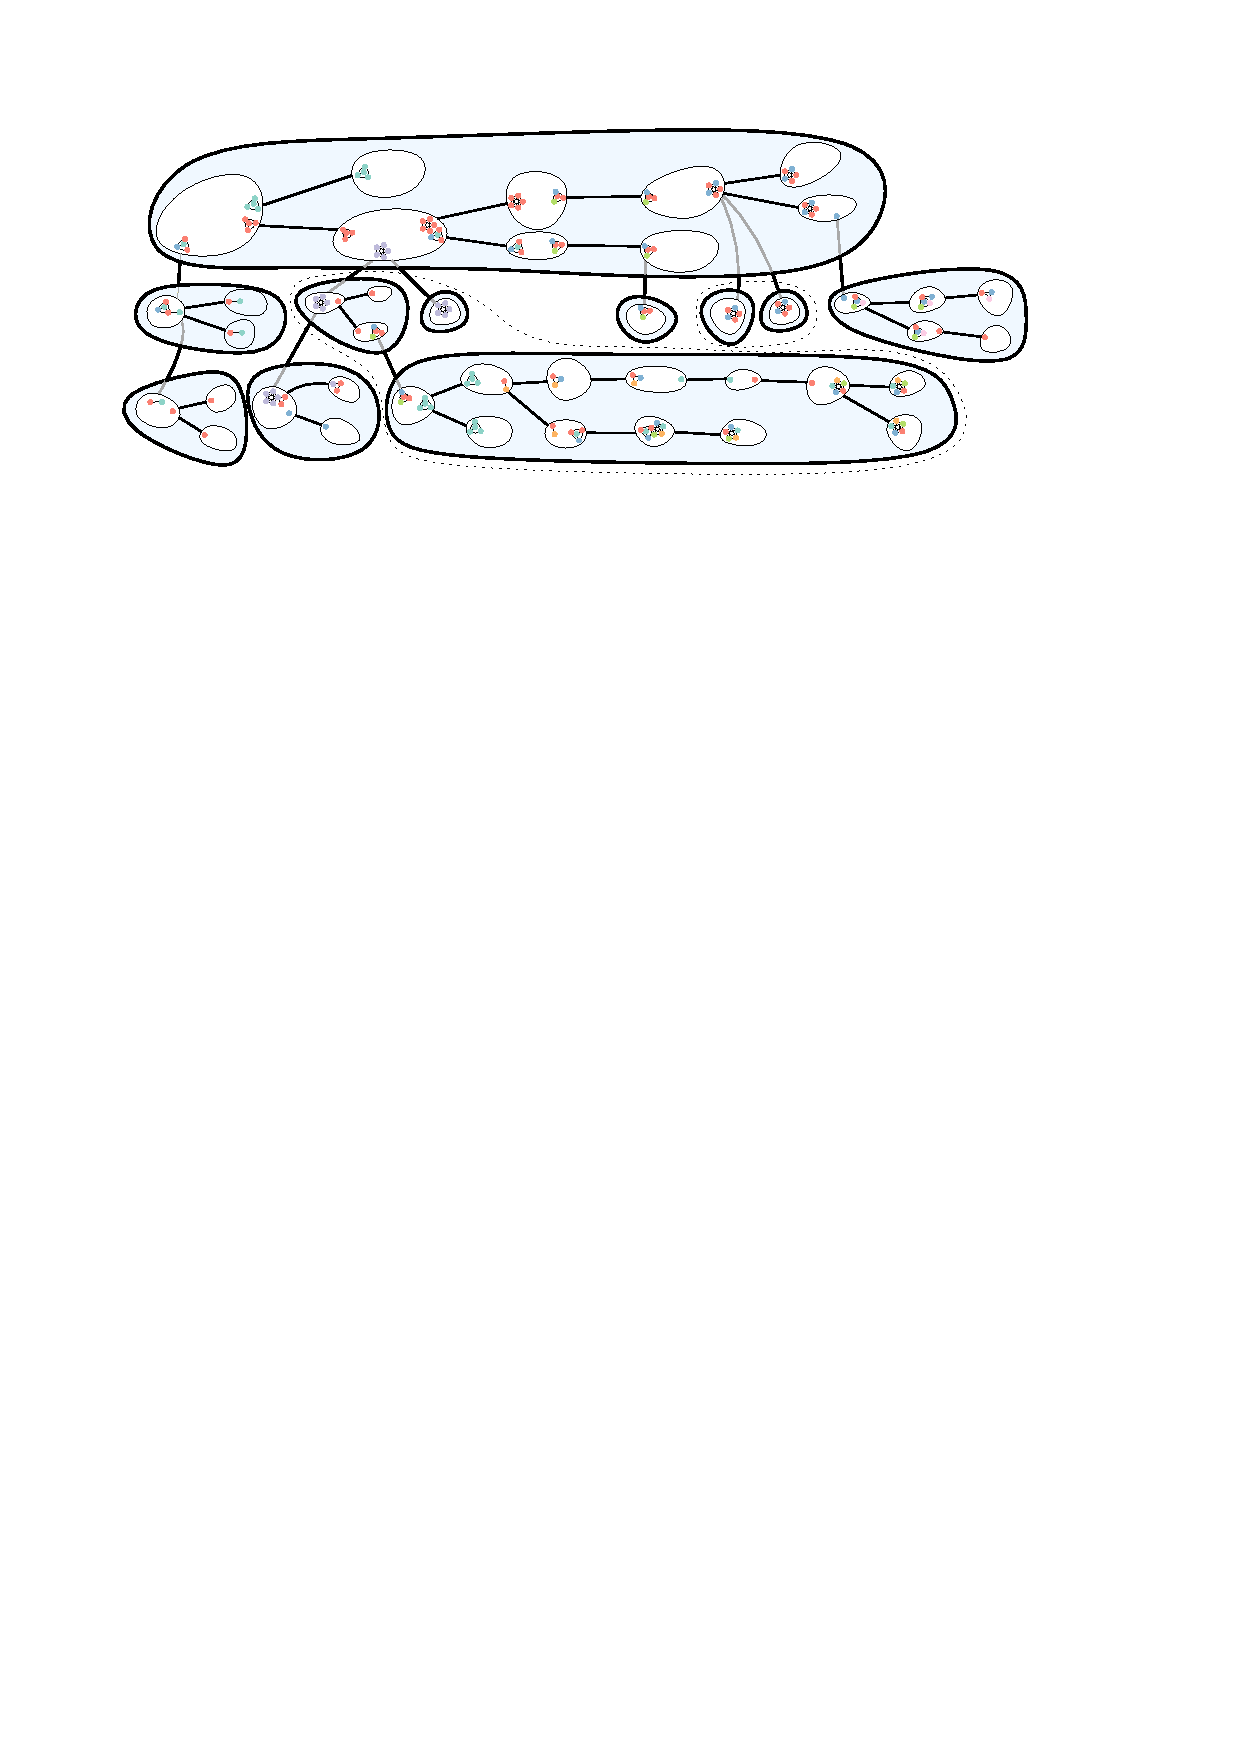
\includegraphics[page=1,width=0.95\textwidth]{figs/t_tprime.pdf} \\[-3ex]
    $\calT$ \\[4ex]
    \includegraphics[page=2,width=0.95\textwidth]{figs/t_tprime.pdf} \\[4ex]
    \includegraphics[page=5,width=0.95\textwidth]{figs/t_tprime.pdf} \\[0ex]
    $\calT'$
  \end{center}
  \caption{    An arbitrary tree-decomposition (top) is refined into a new tree-decomposition in which every bag inherits a tree-decomposition that is skinny (middle), and whose indexing tree, obtained by contracting the bags, has small height (bottom).
  }
  \label{overview_fig}
\end{figure}

Specifically, we propose a simple algorithm that refines an arbitrary (rooted) tree-decomposition into
a 'short' tree-decomposition
such that the adhesion-width stays the same and
all its torsos admit a 'skinny' tree-decomposition and all the adhesions of these new tree-decompositions are adhesions of the original tree-decomposition. See \cref{overview_fig}. Let us make it a bit more concrete.
For $b\in\R^+$, a tree $T$ rooted at $r\in V(T)$ is \defin{$b$-skinny},
if $|\set{v\in V(T) \mid \dist_T(r,v)=i}|\le b$ for each $i\in\N$.  A rooted tree-decomposition $(T,(B_x\mid x\in V(T)))$ of a graph $G$ is \defin{$b$-skinny} if $T$ is $b$-skinny.
Below we rewrite the statement of~\cref{b_skinny_decomp}.

\david{Rather than this quote, I prefer to state the result in a theorem environment, and restate it later if needed.}

\begin{quote}
  For every $b>1$, every $n\in\N^+$, every $n$-vertex graph $G$ and every tree-decomposition $\calT:=(T,(B_x\mid x\in V(T)))$ of $G$, there exists a tree-decomposition $\calQ:=(Q,(D_x\mid x\in V(Q)))$ of $G$ such that
  \begin{enumerate}[nosep,nolistsep,label=\rm(\roman*)]
    \item
          each adhesion of $\calQ$ is an adhesion of $\calT$;
    \item for each $q\in V(Q)$, $\torso{G}{\calQ,D_q}$ \gwen{The notation $\torso{G}{\calQ,D_q}$ has not been defined (and is different from the one that is defined)} has a $b$-skinny tree-decomposition $(T(q), (B_y\mid y\in V(T(q))))$ where $T(q)$ is a subtree of $T$; and
    \item $\height(Q)\le \log_b n$.
  \end{enumerate}
\end{quote}

With this refinement in hand we prove \cref{PlainRealMainTechnical} in the following three steps. For clarity of exposition, the bounds described below are intentionally imprecise. In particular, we omit the big $O$ notation around lower order terms.

\begin{enumerate}[label=\rm(\alph*)]
  \item \label{step:union-closed}
        Let $\calG$ be a class of graphs.
        Let $\calG'$ be the class of graphs that can be formed by taking the union of a finite number of pairwise vertex-disjoint graphs in $\calG$.
        Suppose that $\calG$ admits a $\log n + p(n)$-bit labelling scheme, where $p(n)\in o(\log n)$, show that $\calG'$ admits a $(1+o(1))\log n$-bit labelling scheme, as proved in \cref{disjoint_union_ii}.    If  $\calG$ is a class of graphs that admits a product structure, the result by \citet{dujmovic.esperet.ea:adjacency} states that $\calG$ admits a $\log n + p(n)$-bit labelling scheme where $p(n)\leq \sqrt{\log n}$. \cref{disjoint_union_ii} thus implies $\calG'$  admits $\log n + p(n)$-bit
        \gwen{Shouldn't this be $(1+o(1))\log n$-bit? this would imply changes in the steps below} labelling scheme where $p(n)\leq \sqrt{\log n}$.

  \item \label{step:skinny-tree-decomposition}
        Let $\calG$ be a hereditary class of graphs closed under taking disjoint union.
        Let $k\in\N$ and $b:\N\to\R^+$ be a function with $b(n)>1$ for all $n$.
        Let $\calG'$ be the class of graphs consisting of, for each $n\in\N$, every $n$-vertex graph $G$ with a rooted $b(n)$-skinny tree-decomposition of adhesion-width at most $k$ in which each torso is a member of $\calG$.
        Suppose that $\calG$ admits a $\log n + p(n)$-bit labelling scheme.
        We show that $\calG'$ admits a $\log n +\log b(n) + p(n)$-bit labelling scheme. See~\cref{skinny_labelling}.
  \item \label{step:short-tree-decompositions}
        Let $\calG$ be a hereditary class of graphs closed under taking disjoint union.
        Let $k\in\N$ and  $h:\N\to\R$ be a function with $h(n)\in \Oh(\log n)$ and with $h(n)>0$ for all $n$.
        Let $\calG'$ be the class of graphs consisting of, for each $n\in\N$, every $n$-vertex graph $G$ with a rooted tree-decomposition $\calF:=(F,(B_x \mid x\in V(F)))$ such that
        \begin{enumerate}[nosep,nolistsep,label=(\rm{\roman*)}]
          \item $\calF$ has adhesion-width at most $k$;
          \item $\height(F)\le h(n)$;
          \item for each node $x$ in $F$, the torso $\torso{G}{\calF,B_x}$ \gwen{again, notation undefined} belongs to $\calG$.
        \end{enumerate}
        Suppose that $\calG$ admits a $\log n +\log b(n) + p(n)$-bit labelling scheme.
        We show that $\calG'$ admits a $\log n +\log b(n) + h(n)\cdot p(n)$-bit labelling scheme, thus $\log n + \log b(n) + p(n)\cdot(\log_b n)$-bit labelling scheme. See~\cref{small_height}.
\end{enumerate}

The labelling scheme resulting from these steps has length at most \[
\log n +\log b(n) + h(n)\cdot p(n) \leq \log n +\log b(n) + h(n)\cdot \sqrt{\log n} \enspace.
\]

The lower order terms are minimized by fixing $b:\N\to\R^+$ to be
\[
  b(n):= 2^{(\log n)^{3/4}}.
\]
Thus, the height of the resulting short tree-decomposition in step~\ref{step:short-tree-decompositions} becomes
\[
  h(n) \leq \log_{b(n)}n = \frac{\log n}{(\log n)^{3/4}} = (\log n)^{1/4} \enspace.
\]

All together this gives a labelling scheme of desired length 
\[\log n + O(\log n)^{3/4}\in (1 + o(1))\log n\enspace.\]

%The discussion so far leaves out an important detail of the proof. In order to construct a labelling scheme in step~\ref{step:short-tree-decompositions}, we need to maintain a stronger labelling scheme. For this purpose we develop the notion of a mixed $(g_1,g_2,g_3)$ weighted labelling scheme, where $g_i$ with $i\in[3]$ are functions controlling the size of a lower order term of the label lengths. This definition is a generalization of adjacency labelling schemes. It supports vertex weights and, more importantly, also assigns labels to cliques. Below we proceed with the formal definition.

%Let $\calG$ be a class of graphs. Let $g_i:\N\to\R^+$ for each $i\in[3]$. The class  $\calG$ admits a \defin{weighted $(g_1,g_2,g_3)$ mixed labelling scheme} of $\calG$ if there exists a pair $(A,I)$ with \begin{itemize}[nosep,nolistsep]     \item $A:(\{0,1\}^*)^2\to\{0,1\}$ (the \defin{adjacency tester}); and     \item $I:(\{0,1\}^*)^3\to\{0,1\}$ (the \defin{identity tester}) \end{itemize} such that for every natural $n\in\N$, every $n$-vertex graph $G^+$ in $\calG$, every spanning subgraph $G$ of $G^+$, and every weight function $\omega:V(G)\to \R^+$, there exists an injective function $\mu: V(G)\cup K(G^+) \to \set{0,1}^*$ and a function $\kappa:\{(K, u)\mid \textrm{$K$ clique in $G^+$}, u\in K\}\to \set{0,1}^*$ such that \begin{enumerate}[nosep,nolistsep,label=(\roman*)]    \item for all $u,v\in V(G)$,    \[\textrm{$A(\mu(u),\mu(v))=1$ if and only if $uv\in E(G)$;}    \] \item for every clique $K$ in $G^+$, $u\in K$, $v\in V(G)$,    \[\textrm{$I(\mu(K),\kappa(K, u),\mu(v))=1$ if and only if $u=v$;}   \]\item for every $v\in V(G)$, \[   |\mu(v)| \leq \log \omega(G) - \log\omega(v) + g_1(n); \]       \item for every clique $K$ in $G^+$,\[    |\mu(K)|\le \log \omega(G) - \log\min_{v\in K}(\omega(v)) + g_3(n);   \]\item  for every clique $K$ in $G^+$ and $u\in K$,    \[|\kappa(K, u)| \leq g_2(n).    \] \end{enumerate}
%Given $\mu$ and $\kappa$  as above we say that $(\mu,\kappa)$ is a \defin{mixed labelling} of $(G^+,G,\omega)$ for $(A,I)$.

%Function $g_1(n)$ measures how much the length of a vertex label exceeds the ideal value $\log \omega(G) - \log\omega(v)$ that appears in Kraft's Inequality \cite{Kraft1949}. Function $g_3(n)$ measures how much the length of a clique label exceeds the Kraft-like quantity $\log\min_{v\in K}(\omega(v))$.  Function $g_2(n)$ is the length of the longest local identifier.


%Again, we stress that this 
\david{revise this paragraph}
The generalization of adjacency labelling scheme
to the mixed weighting setting
is introduced to complete the proof in step~\ref{step:short-tree-decompositions}.  In particular, the class $\calG$ given as input to step~\ref{step:short-tree-decompositions} must admit a weighted $(g_1,g_2,g_3)$ mixed labelling scheme with $g_i\in o(\log n)$ for each $i\in[3]$.  This requires that we describe weighted mixed labelling schemes for the graph classes $\calG'$ that appear in steps~\ref{step:apex}, \ref{step:union-closed}, and \ref{step:skinny-tree-decomposition}.  It also requires that we generalize the adjacency labelling scheme for $\calG_k$ given by~\citet{dujmovic.esperet.ea:adjacency} to obtain a weighted mixed labelling scheme for graphs in $\calG_k$.
This generalization, which is discussed in \cref{weighted_product_proof}, is fairly straightforward: The notion of clique labels and membership labels is already implicit in \cite{dujmovic.esperet.ea:adjacency} and the addition of vertex weights is accomplished by a  standard trick of simulating weight by multiplicity.

Step~\ref{step:union-closed} follows using a basic trick with weighted labels.
For clarity, we explain here only how to maintain the labels for adjacency tester.
Let $G^+$ be an $n$-vertex graph in $\calG'$ and let $G$ be a spanning subgraph of $G$.
\gwen{of $G^+$?}
Thus,
$G^+=\bigcup_{i\in[m]}G^+_i$ where $G^+_i\in\calG$ for each $i\in[m]$.
Let $G_i=G[V(G^+_i)]$ for each $i\in[m]$.
Let $\omega: V(G)\to\N^+$ (by an easy reduction we may assume that weights are positive integers).
Let $\psi:[m]\to\N^+$ be the weight function defined by $\psi(i):=\omega(G_i)$.
Classical construction of prefix-free codes,
see~\cref{shannon_fano_elias_code}, applied to the set $[m]$ with weight function $\psi$
results in a prefix-free code $\rho:[m]\to\{0,1\}^*$ such that for each $i\in[m]$ we have
\[
  |\rho(i)|\le\log \omega(G)-\log \omega(G_i)+3\enspace.
\]
For each $i\in[m]$,
let $\mu_i$ be the labelling of $(G_i^+,G_i,\omega_{|V(G_i)})$ in the scheme for $\calG$.
Thus, for each $i\in[m]$ and each $v\in V(G_i)$,
\[
  |\mu_i(v)| \le \log\omega(G_i) - \log\omega(v) + g_1(n)\enspace.
\]
The final label of a vertex is a simple concatenation of $\rho$ and $\mu_i$.
For each $i\in[m]$, each $v\in V(G_i)$, let
$\mu(v):=(\rho(i),\mu_i(v))$.
We can see that the length of the label $\mu(v)$ is at most $\log\omega(G)-\log\omega(v)+g_1(n)$ plus a small surplus.
(Again we ignored here the cost of decoding a concatenation.)

We employ two orthogonal strategies to devise labellings in steps~\ref{step:skinny-tree-decomposition} and~\ref{step:short-tree-decompositions}.
This is the main conceptual and technical contribution of this paper.
In the setup of step~\ref{step:skinny-tree-decomposition},
we project a given skinny tree-decomposition to a path-decomposition and setup a labelling scheme there.
In the setup of step~\ref{step:short-tree-decompositions}, we are given a short tree-decomposition.
We will root this tree and the final label of vertex $v$ will be a concatenation of labels of adhesion cliques starting from the root bag up to the first bag $B$ containing $v$,
together with the label of $v$ in $G[B]$ the scheme for $\calG$.
The bounds on the label lengths will guarantee that the total length of this concatenation will be bounded by $\log\omega(G)-\log\omega(v)$ plus a lower order term.
The label will include extra bits of information but they will only contribute to the lower order term in the final length.



% \piotr{New version. Unfinished.}
% \begin{comment}
% \subsection{Proof Overview (Piotrek)}

% The \defin{strong product} of graphs~$A$ and~$B$, denoted by~${A \boxtimes B}$, is the graph with vertex-set ${V(A) \times V(B)}$, where distinct vertices ${(v,x),(w,y) \in V(A) \times V(B)}$ are adjacent if
% ${v=w}$ and ${xy \in E(B)}$, or
% ${x=y}$ and ${vw \in E(A)}$, or
% ${vw \in E(A)}$ and~${xy \in E(B)}$.
% For an integer $k\geq 0$, let \defin{$\calG_{k}$} be the class of graphs isomorphic to a subgraph of $H\boxtimes P$ for some graph $H$ with treewidth at most $k$ and for some path $P$.
% A class of graphs $\calG$ admits a \defin{product structure},
% if there exists an integer $k$ such that $\calG\subseteq \calG_k$.
% As mentioned in the introduction,
% only apex-minor-free classes admit a  product structure.
% Since we aim to deal with an arbitrary proper minor-closed class of graphs, we need to step back and rely on a much weaker structural description.
% For integers $k,a\geq 0$, let \defin{$\calG_{k,a}$} be the class of graphs that are isomorphic to a graph in $\calG_k$ after removing at most $a$ vertices.
% The following statement, sometimes called the graph minor product structure theorem,  proved by~\citet{dujmovic.joret.ea:planar} is the foundation stone for our labelling scheme:
% \begin{quote}
%   For every proper minor-closed class $\calG$ there exist integers $k,a\geq 0$ such that every graph in $\calG$ has a tree-decomposition in which every torso is in $\calG_{k,a}$.
% \end{quote}

% On the adjacency labelling side, we start with
% the $(1+o(1))$-bit adjacency labelling scheme for $\calG_k$ given by
% \citet{dujmovic.esperet.ea:adjacency}.
% Therefore, all one needs to do to complete a proof of~\cref{main_result}
% are the following two steps:
% \begin{enumerate}[label=\rm(\arabic*)]
%   \item \label{step:apex} Let $\calG$ be a class of graphs and $a\in\N$.
%         Let $\calG'$ be the class of graphs consisting of
%         every graph obtained from a graph in $\calG$
%         by adding at most $a$ vertices and
%         adding arbitrary edges incident to the new vertices.
%         Suppose that $\calG$ admits a $(1+o(1))\log n$-bit labelling scheme.
%         Show that $\calG'$ admits a $(1+o(1))\log n$-bit labelling scheme.
%   \item Let $\calG$ be a class of graphs and $k\in\N$.
%         Let $\calG'$ be the class of graphs consisting of, for each $n\in\N$, every $n$-vertex graph $G$ with a tree-decomposition of adhesion-width at most $k$ in which each torso is a member of $\calG$.
%         Suppose that $\calG$ admits a $(1+o(1))\log n$-bit labelling scheme.
%         Show that $\calG'$ admits a $(1+o(1))\log n$-bit labelling scheme.
% \end{enumerate}

% The first step concerning adding apices is relatively straightforward.
% Let $G$ be a graph in $\calG'$ and
% let $X$ be a subset of vertices of $G$ with $|X|\leq a$ such that $G-X$ is in $\calG$.
% We construct the labelling of vertices of $G$ as follows.
% For each vertex $v$,
% the label $\mu(v)$ of $v$ has three parts $(\sigma(v),c(v),\mu^-(v))$,
% where $\sigma(v)$ is an identifier that tells if $v$ is an apex vertex (i.e., if $v\in X$) and if so it records the identifier of $v$;
% $c(v)$ records the adjacency status of $v$ with each of the apices; and
% finally $\mu^-(v)$, which is defined only if $v\in V(G-X)$, is the label of $v$ in the adjacency labelling scheme of $G-X$ in $\calG$.
% It is rather clear that given two such labels $\mu(v)$, $\mu(w)$ of vertices $v$, $w$ in $G$, the adjacency tester is able to decide whether $v$ and $w$ are adjacent in $G$.
% Also the length of a label has increased by at most $\Oh(a)$-bits comparing to labels in the scheme for $\calG$.
% (In this overview we omit a discussion on the extra cost incurred to be able to decode concatenation of labels of various lengths.)
% All this is essentially the content of the proof of~\cref{add_apexes}.

% Unfortunately, we do not see an easy way to complete the second step.
% Instead, we do the following.
% We propose a simple algorithm refining an arbitrary (rooted) tree-decomposition into
% a 'short' tree-decomposition
% such that the adhesion-width stays the same and
% all its torsos admit a 'skinny' tree-decomposition and all the adhesions of these new tree-decompositions are adhesions of the original tree-decomposition. Let us make it a bit more concrete.
% For $b\in\R^+$, a tree $T$ rooted at $r\in V(T)$ is \defin{$b$-skinny},
% if $|\set{v\in V(T) \mid \dist_T(r,v)=i}|\le b$ for each $i\in\N$.  A rooted tree-decomposition $(T,(B_x\mid x\in V(T)))$ of a graph $G$ is \defin{$b$-skinny} if $T$ is $b$-skinny.
% Below we rewrite the statement of~\cref{b_skinny_decomp}.

% \begin{quote}
%   For every $b>1$, every $n\in\N^+$, every $n$-vertex graph $G$ and every tree-decomposition $\calT:=(T,(B_x\mid x\in V(T)))$ of $G$, there exists a tree-decomposition $\calQ:=(Q,(D_x\mid x\in V(Q)))$ of $G$ such that
%   \begin{enumerate}[nosep,nolistsep,label=\rm(\roman*)]
%     \item
%           each adhesion of $\calQ$ is an adhesion of $\calT$;
%     \item for each $q\in V(Q)$, $\torso{G}{\calQ,D_q}$ has a $b$-skinny tree-decomposition $(T(q), (B_y\mid y\in V(T(q))))$ where $T(q)$ is a subtree of $T$; and
%     \item $\height(Q)\le \log_b n$.
%   \end{enumerate}
% \end{quote}

% With this refinement in hand we execute step two in the following three substeps.

% \begin{enumerate}[label=\rm(2\alph*)]
%   \item \label{step:union-closed}
%         Let $\calG$ be a class of graphs.
%         Let $\calG'$ be the class of graphs that can be formed by taking the union of a finite number of pairwise vertex-disjoint graphs in $\calG$.
%         Suppose that $\calG$ admits a $(1+o(1))\log n$-bit labelling scheme.
%         Show that $\calG'$ admits a $(1+o(1))\log n$-bit labelling scheme. See~\cref{disjoint_union_ii}.
%   \item \label{step:skinny-tree-decomposition}
%         Let $\calG$ be a hereditary class of graphs closed under taking disjoint union.
%         Let $k\in\N$ and $b:\N\to\R^+$ be a function with $b(n)>1$ for all $n$.
%         Let $\calG'$ be the class of graphs consisting of, for each $n\in\N$, every $n$-vertex graph $G$ with a rooted $b(n)$-skinny tree-decomposition of adhesion-width at most $k$ in which each torso is a member of $\calG$.
%         Suppose that $\calG$ admits a $(1+o(1))\log n$-bit labelling scheme.
%         Show that $\calG'$ admits a $(1+o(1))\log n$-bit labelling scheme. See~\cref{skinny_labelling}.
%   \item \label{step:short-tree-decompositions}
%         Let $\calG$ be a hereditary class of graphs closed under taking disjoint union.
%         Let $k\in\N$ and  $h:\N\to\R$ be a function with $h(n)\in \Oh(\log n)$ and with $h(n)>0$ for all $n$.
%         Let $\calG'$ be the class of graphs consisting of, for each $n\in\N$, every $n$-vertex graph $G$ with a rooted tree-decomposition $\calF:=(F,(B_x \mid x\in V(F)))$ such that
%         \begin{enumerate}[nosep,nolistsep,label=(\rm{\roman*)}]
%           \item $\calF$ has adhesion-width at most $k$;
%           \item $\height(F)\le h(n)$;
%           \item for each node $x$ in $F$, the torso $\torso{G}{\calF,B_x}$ belongs to $\calG$.
%         \end{enumerate}
%         Suppose that $\calG$ admits a $(1+o(1))\log n$-bit labelling scheme.
%         Show that $\calG'$ admits a $(1+o(1))\log n$-bit labelling scheme. See~\cref{small_height}.
% \end{enumerate}

% In the final argument, we fix $b:\N\to\R^+$ to be
% \[
%   b(n):= 2^{(\log n)^{3/4}}.
% \]
% Thus, the height of the resulting 'short' tree-decomposition becomes
% \[
%   h(n) \leq \log_{b(n)}n = \frac{\log n}{(\log n)^{3/4}} = (\log n)^{1/4}.
% \]

% The discussion so far leaves out an important detail of the proof. In order to construct a labelling scheme in step~\ref{step:short-tree-decompositions},
% we need to maintain a stronger labelling scheme.
% For this purpose we develop the notion of a mixed $(g_1,g_2,g_3)$ weighted labelling scheme, where $g_i$ with $i\in[3]$ are functions controlling the size of a lower order term of the label lengths.
% This definition is a generalization of adjacency labelling schemes.
% It supports vertex weights and, more importantly, also assigns labels to cliques. Below we proceed with the formal definition.

% Let $\calG$ be a class of graphs.
% Let $g_i:\N\to\R^+$ for each $i\in[3]$.
% The class  $\calG$ admits a \defin{weighted $(g_1,g_2,g_3)$ mixed labelling scheme} of $\calG$ if there exists a pair $(A,I)$ with
% \begin{itemize}[nosep,nolistsep]
%   \item $A:(\{0,1\}^*)^2\to\{0,1\}$ (the \defin{adjacency tester}); and
%   \item $I:(\{0,1\}^*)^3\to\{0,1\}$ (the \defin{identity tester})
% \end{itemize}
% such that
% for every natural $n\in\N$,
% every $n$-vertex graph $G^+$ in $\calG$,
% every spanning subgraph $G$ of $G^+$, and
% every weight function $\omega:V(G)\to \R^+$,
% there exists an injective function $\mu: V(G)\cup K(G^+) \to \set{0,1}^*$ and a function $\kappa:\{(K, u)\mid \textrm{$K$ clique in $G^+$}, u\in K\}\to \set{0,1}^*$
% such that
% \begin{enumerate}[nosep,nolistsep,label=(\roman*)]
%   \item for all $u,v\in V(G)$
%         \[
%           \textrm{$A(\mu(u),\mu(v))=1$ if and only if $uv\in E(G)$;}
%         \]
%   \item for every clique $K$ in $G^+$, $u\in K$, $v\in V(G)$
%         \[
%           \textrm{$I(\mu(K),\kappa(K, u),\mu(v))=1$ if and only if $u=v$;}
%         \]
%   \item for every $v\in V(G)$
%         \[
%           |\mu(v)| \leq \log \omega(G) - \log\omega(v) + g_1(n);
%         \]
%   \item for every clique $K$ in $G^+$,
%         \[
%           |\mu(K)|\le \log \omega(G) - \log\min_{v\in K}(\omega(v)) + g_3(n);
%         \]
%   \item  for every clique $K$ in $G^+$ and $u\in K$
%         \[
%           |\kappa(K, u)| \leq g_2(n).
%         \]
% \end{enumerate}
% Given $\mu$ and $\kappa$  as above we say that $(\mu,\kappa)$ is a \defin{mixed labelling} of $(G^+,G,\omega)$ for $(A,I)$.

% Again, we stress that this generalization of adjacency labelling scheme is introduced to complete the proof in step~\ref{step:short-tree-decompositions}.  In particular, the class $\calG$ given as input to step~\ref{step:short-tree-decompositions} must admit a weighted $(g_1,g_2,g_3)$ mixed labelling scheme with $g_i\in o(\log n)$ for each $i\in[3]$.  This requires that we describe weighted mixed labelling schemes for the graph classes $\calG'$ that appear in steps~\ref{step:apex}, \ref{step:union-closed}, and \ref{step:skinny-tree-decomposition}.  It also requires that we generalize the adjacency labelling scheme for $\calG_k$ given by~\citet{dujmovic.esperet.ea:adjacency} to obtain a weighted mixed labelling scheme for graphs in $\calG_k$.
% This generalization, which is discussed in \cref{weighted_product_proof}, is fairly straightforward: The notion of clique labels and membership labels is already implicit in \cite{dujmovic.esperet.ea:adjacency} and the addition of vertex weights is accomplished by a  standard trick of simulating weight by multiplicity.


% The step~\ref{step:union-closed} follows by thanks to a basic trick with weighted labels.
% For clarity, we explain here only how to maintain the labels for adjacency tester.
% Let $G^+$ be an $n$-vertex graph in $\calG'$ and let $G$ be a spanning subgraph of $G$.
% Thus,
% $G^+=\bigcup_{i\in[m]}G^+_i$ where $G^+_i\in\calG$ for each $i\in[m]$.
% Let $G_i=G[V(G^+_i)]$ for each $i\in[m]$.
% Let $\omega: V(G)\to\N^+$ (by an easy reduction we may assume that weights are positive integers).
% Let $\psi:[m]\to\N^+$ be the weight function defined by $\psi(i):=\omega(G_i)$.
% Classical construction of prefix-free codes,
% see~\cref{shannon_fano_elias_code}, applied to the set $[m]$ with weight function $\psi$
% results in a prefix-free code $\rho:[m]\to\{0,1\}^*$ such that for each $i\in[m]$ we have
% \[
%   |\rho(i)|\le\log \omega(G)-\log \omega(G_i)+3\enspace.
% \]
% For each $i\in[m]$,
% let $\mu_i$ be the labelling of $(G_i^+,G_i,\omega_{|V(G_i)})$ in the scheme for $\calG$.
% Thus, for each $i\in[m]$ and each $v\in V(G_i)$,
% \[
%   |\mu_i(v)| \le \log\omega(G_i) - \log\omega(v) + g_1(n)\enspace.
% \]
% The final label of a vertex is a simple concatenation of $\rho$ and $\mu_i$.
% For each $i\in[m]$, each $v\in V(G_i)$, let $\mu(v)=(\rho(i),\mu_i(v))$.
% We can see that the length of the label $\mu(v)$ is at most $\log\omega(G)-\log\omega(v)+g_1(n)$ plus a small surplus.
% (Again we ignored here the cost of decoding a concatenation.)


% We employ two orthogonal strategies to devise labellings in steps~\ref{step:skinny-tree-decomposition} and~\ref{step:short-tree-decompositions}.
% This is the main conceptual and technical contribution of this paper.
% In the setup of step~\ref{step:skinny-tree-decomposition},
% we project a given skinny tree-decomposition to a path-decomposition and setup a labelling scheme there.
% In the setup of step~\ref{step:short-tree-decompositions}, we are given a short tree-decomposition.
% We are going to root this tree and the final label of vertex $v$ is going to be a concatenation of labels of adhesion cliques starting from the root bag up to the first bag $B$ containing $v$,
% together with the label of $v$ in $G[B]$ the scheme for $\calG$.
% The bounds on the label lengths will guarantee that the total length of this concatenation will be bounded by $\log\omega(G)-\log\omega(v)$ plus a lower order term.
% The label will consist extra bits of information but they will only contribute to the lower order term in the final length.

% \end{comment}

% \begin{comment}
% \piotr{Old version}
% \subsection{Proof Overview (Pat)}
% \label{ssec:overview}


% We prove \cref{main_result} by introducing a new generalization of adjacency labelling, called weighted mixed labelling. It supports vertex weights and, more importantly, also assigns labels to cliques. These labellings are defined for vertex-weighted graphs in which each vertex $v$ is assigned a positive integer weight $\omega(v)$.  A \defin{weighted mixed labelling} is defined in terms of a graph $G^+$ equipped with a weight function $\omega$, a spanning subgraph $G$ of $G^+$, and a subset $\calK$ of the cliques in $G^+$. A mixed labelling of $(G^+,G,\calK,\omega)$ is then a function $\mu:V(G^+)\cup\calK\to\{0,1\}^*$ that assigns a label to each vertex of $G^+$ and each clique in $\calK$.  In addition to this, for each clique $K\in\calK$, each vertex $v$ in $K$ is assigned a label $\kappa(K,v)$ called the \defin{local identifier} for $v$ in $K$.

% Let $\Omega:=\sum_{v\in V(G^+)}\omega(v)$ be the total weight of vertices in $G^+$.  The efficiency of a mixed labelling is measured by three parameters
% \begin{itemize}
%   \item $g_1=\max_{v\in V(G^+)} (|\mu(v)|-(\log\Omega - \log\omega(v)))$ measures how much the length of a vertex label exceeds the ideal value $\log\Omega-\log\omega(v)$ that appears in Kraft's Inequality \cite{Kraft1949}.
%   \item $g_2=\max\{\kappa(K,v):K\in\calK, v\in K\}$ is the length of the longest local identifier.
%   \item $g_3=\max_{K\in\calK} (|\mu(K)|-(\log\Omega - \log(\min_{v\in K}\omega(v))))$ measures how much the length of a clique label exceeds the Kraft-like quantity $\log\Omega - \log(\min_{v\in K}\omega(v)))$.
% \end{itemize}


% Mixed labellings generalize adjacency labellings: Any two vertex labels $\mu(v)$ and $\mu(w)$ are sufficient to perform an adjacency test between the vertices $v$ and $w$ in the subgraph $G$.  In addition to this, for any clique $K$ in $\calK$, any vertex $v'$ of $G^+$, and any vertex $v$ of $K$, the labels $\mu(K)$, $\mu(v')$ and $\kappa(K,v)$ are sufficient to test if $v'=v$.  The idea here is that $\kappa(K,v)$ provides each vertex $v$ in $K$ a short label that is only useful when $\mu(K)$ is also available.   A mixed labelling scheme $\mu$ is \defin{efficient} if $g_1,g_2,g_3\in o(\log n)$.  Note that, if we use the uniform weighting $\omega(v)=1$ for each $v\in V(G)$, then all labels in an efficient mixed labelling have length $(1+o(1))\log n$.  In particular, such a labelling is a $((1+o(1))\log n)$-bit adjacency labelling of $G$.

% Our main technical result, from which \cref{main_result} quickly follows, is stated in terms of tree-decompositions.  A \defin{tree-decomposition} of a graph $G$ is a pair $(T,(B_x \mid x \in V(T)))$,
% where $T$ is a tree and $B_x \subseteq V(G)$ for every $x \in V(T)$, with the
% following properties:
% \begin{enumerate*}[label=(\alph*)]
%   \item for each vertex $u$ in $G$, the subgraph of $T$ induced by $\{x \in V(T) \mid u \in B_x\}$ is non-empty and connected; and
%   \item for each edge $uv$ in $G$, there exists $x\in V(T)$ such that $u,v\in B_x$.
% \end{enumerate*}
% We call the sets $B_x$ the \defin{bags} of the tree-decomposition and the sets $B_x\cap B_y$ for all distinct $x,y\in V(T)$, the \defin{adhesions} of the tree-decomposition.
% The \defin{width} of a tree-decomposition is the maximum size of a bag minus one.
% The \defin{adhesion-width} of a tree-decomposition is the maximum size of an adhesion.

% Let $G$ be a graph,
% let $\calT=(T,(B_x \mid x\in V(T)))$ be a tree-decomposition of $G$, and let $x$ be a vertex of $T$.
% The \defin{torso} of $x$, denoted \defin{$\torso{G}{\calT,B_x}$},
% is the graph with the vertex-set $B_x$ in which two distinct vertices $u$ and $v$ are adjacent
% if $uv \in E(G)$, or there exists $y \in N_T(x)$  such that $u,v \in B_x \cap B_y$.\footnote{For a graph $G$ and a vertex $v$ of $G$, $N_G(v)$ denotes a set of neighbours of $v$ in $G$. The notation $\torso{G}{B_x}$ introduces some minor ambiguity since the definition of $\torso{G}{B_x}$ depends on $(B_y:y\in N_T(x))$, but the notation makes no reference to the tree-decomposition $(T, (B_z\mid z\in V(T))$.  When we use this notation, the tree-decomposition will always be obvious from context.}
% A tree-decomposition $(T,(B_x \mid x\in V(T)))$ is \defin{rooted} if $T$ is a rooted tree.  The \defin{home node} of a vertex $v$ of $G$ in a rooted tree-decomposition $(T,(B_x \mid x\in V(T)))$ is the minimum-depth node $x$ of $T$ such that $v\in B_x$.  The \defin{parent adhesion} of a node $x$ in $T$ is the set of vertices in $B_x$ whose home bag is not $x$.  The \defin{lower torso} at $x$ is the subgraph of $\torso{G}{B_x}$ that is left after removing vertices in the parent adhesion of $x$. A fundamental property of tree-decompositions is that, for any edge $vw$ of $G$, the home nodes of $v$ and $w$ are in an ancestor-descendant relationship in $T$ (including the possibility that $v$ and $w$ have the same home node).

% A graph class $\calG$ is \defin{hereditary} if, for every $G\in\calG$, every induced subgraph of $G$ is in $\calG$. We can now state our main technical result:
% \begin{thm}\label{PlainRealMainTechnical}
%   Let $\calG$ be a hereditary graph class that admits an efficient weighted mixed labelling scheme. Then, for any fixed $k$, the family $\calG'$ of all graphs having tree-decomposition of adhesion-width at most $k$ whose torsos are in $\calG$ also admits an efficient weighted mixed labelling scheme.
% \end{thm}
% % \pat{TODO: Switch from $\calT'$ and $T'$ to $\calQ$ and $Q$, to be consistent with the revised version of \cref{b_skinny_decomp}.} \vida{I am not sure about that, as at this stage using T and T' is very natural.}

% The proof of \cref{PlainRealMainTechnical} has a relatively simple high-level description, illustrated in \cref{overview_fig}.  The first step is to partition the vertices of the tree $T$ indexing a tree-decomposition $\calT$ into `skinny' subtrees so that contracting each of these subtrees gives a `short' tree $T'$ (\cref{b_skinny_decomp}).  Here, the skinnyness of subtrees and the shortness of $T'$ share a common parameter \defin{$b$} where increasing $b$ makes $T'$ shorter (decreases the height of $T'$) but makes the subtrees in the partition less skinny.  One can then treat $T'$ as indexing a tree-decomposition $\calT'$ of $G$ whose torsos: (a) have skinny tree-decompositions (each defined by one of the subtrees in the partition); and, (b) admit efficient weighted mixed labelling schemes.

% \begin{figure}
%   \begin{center}
%     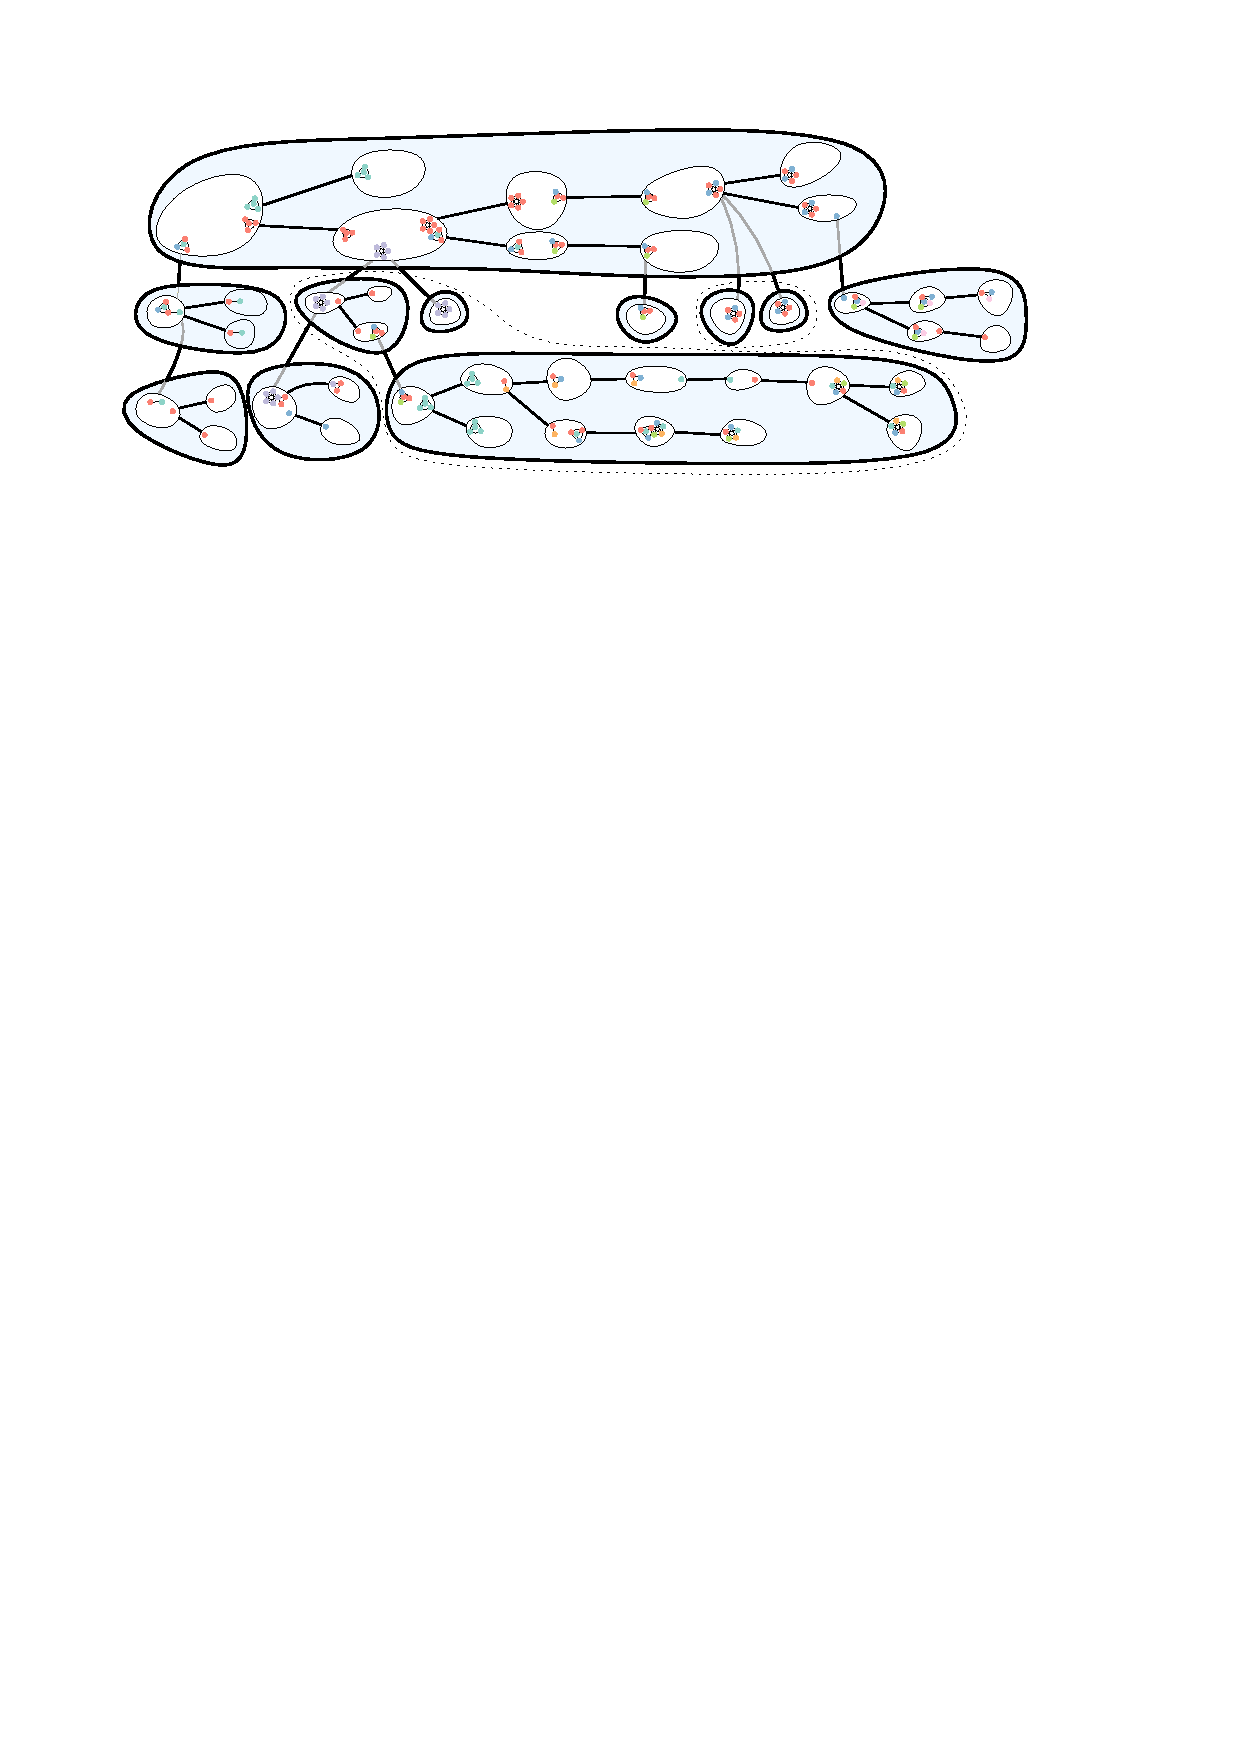
\includegraphics[page=1,width=0.95\textwidth]{figs/t_tprime.pdf} \\[-3ex]
%     $\calT$ \\[4ex]
%     \includegraphics[page=2,width=0.95\textwidth]{figs/t_tprime.pdf} \\[4ex]
%     \includegraphics[page=5,width=0.95\textwidth]{figs/t_tprime.pdf} \\[0ex]
%     $\calT'$
%   \end{center}
%   \caption{The proof of \cref{PlainRealMainTechnical} works by partitioning the tree $T$ indexing a tree-decomposition $\calT$ (top) into skinny subtrees (middle) so that contracting these gives a short tree $T'$ indexing the tree-decomposition $\calT'$ (bottom).}
%   \label{overview_fig}
% \end{figure}

% The proof then proceeds in two steps: The first step is to show that graphs that have skinny tree-decompositions whose torsos admit efficient weighted mixed labelling schemes also have efficient weighted mixed labelling schemes (\cref{skinny_labelling}). The second shows that graphs that have tree-decompositions of sufficiently small height  whose torsos admit efficient weighted mixed labelling schemes also admit efficient weighted mixed labelling schemes (\cref{small_height}).  These are then combined by partitioning the vertices the tree indexing an arbitrary tree-decomposition of $G$ so that each part induces a skinny subtree, proves a more precise version of \cref{PlainRealMainTechnical} that quantifies the efficiency of the resulting weighted mixed labelling scheme (\cref{RealMainTechnical}).

% The first step of the proof makes use of the fact that a tree-decomposition indexed by a skinny tree $T$ can be linearized to obtain a path decomposition with adhesion-width $\Oh(bk)$. The solution of this path-decomposition-based subproblem involves a combination of techniques that have been developed for similar (though unweighted) problems \cite{gavoille.labourel:shorter,dujmovic.esperet.ea:adjacency}. The extension to the weighted version (and mixed labellings) is achieved by using alphabetic binary trees rather than the balanced binary trees used in \cite{gavoille.labourel:shorter,dujmovic.esperet.ea:adjacency}.  One critical detail  that our construction ensures and the solution makes use of, is that it guarantees more than just the adhesion-width bound \(\Oh(bk)\). In the linearization we use the fact that each vertex has at most $k$ neighbours in the parent adhesion of its home node, and this is important.

% The generalization provided by weighted mixed labelling schemes is crucial for the second step, as we now explain.  Let $w$ be a vertex of $G$ and let $x_0,\ldots,x_s$ be the path from the root $x_0$ of the short tree $T'$ to the home node $x_s$ of $w$.  (Most of) the vertex label $\mu(w)$ is obtained by concatenating the labels $\mu_{x_0}(K_1),\ldots,\mu_{x_{s-1}}(K_s),\mu_{x_s}(w)$ where $\mu_{x_0}$ is a mixed labelling of $\torso{G}{B_{x_0}}$, $\mu_{x_i}$ is a mixed labelling of $\torso{G}{B_{x_i}}-B_{x_{i-1}}$, and $K_i$ is a clique whose vertex-set is contained in the adhesion $B_{x_{i-1}}\cap B_{x_i}$, for each $i\in\{1,\ldots,s\}$.  This serves two purposes:
% \begin{enumerate}
%   \item For two vertices $v$ and $w$, the longest common prefix of $\mu(v)$ and $\mu(w)$ can be used to determine if the home nodes in $\calT'$ for $v$ and $w$ are in an ancestor-descendant relationship (or if $v$ and $w$ have the same home node.)
%   \item The vertex label $\mu(w)$ for $w$ can be augmented to explicitly store $\kappa(K_{x_i},v)$ for each neighbour $v$ of $w$ whose home node is a strict ancestor $x_{i}$ of $w$'s home node $x_{s}$. Each such vertex $v$ is necessarily contained in the adhesion $B_{x_s}\cap B_{x_{s-1}}$.  Since the adhesion-width of $\calT'$ is at most $k$, this adds at most $k\cdot g_2(n)$ to the length of $\mu(w)$.
% \end{enumerate}
% The total length of vertex labels is controlled by using the appropriate weight function $\omega_{x}$ when computing the weighted mixed labelling for the lower torso of each node $x$ of $T'$.


% Despite the simplicity of this high-level description, getting all of this to work involves carefully managing the interplay between the skinnyness parameter $b$, the input parameters $g_1$, $g_2$, and $g_3$ of the weighted mixed labelling scheme for each torso of the original tree-decomposition $\calT$, the parameters $g_1'$, $g_2'$ and $g_3'$ of the weighted mixed labelling scheme for graphs with skinny tree-decompositions, and the parameters $g_1''$, $g_2''$ and $g_3''$ of the weighted mixed labelling scheme for the entire graph. For example, the lengths of the labels $\mu_{x_0}(K_1),\ldots,\mu_{x_{s-1}}(K_s),\mu_{x_s}(w)$ described above form a telescoping series that sums to $\log\Omega - \log\omega(w) + s\cdot g'_3 + g'_1$, so the value of $g_1''$ is at least $s\cdot g'_3 + g'_1$, which is why we require that $T'$ is short, since the height of $T'$ upper bounds $s$.  This requires using a large value of $b$, which makes the subtrees used to define $T'$ less skinny, this increases the value of $g_2'$, which increases the length of the second part of $\mu(w)$, which has length $k\cdot g_2'(n)$.
% Optimizing the trade-off between the skinnyness parameter $b$ and the height $h$ of $T'$ ultimately yields the $\Oh((\log n)^{3/4})$ lower order term in our final bound.


% To deduce \cref{main_result} from \cref{PlainRealMainTechnical}, we use two ingredients.  The first ingredient is a rough
% version of the Robertson-Seymour Graph Minor Structure Theorem due to \citet{dujmovic.joret.ea:planar} which states that every graph in a proper-minor-closed family $\calG$ has a tree-decomposition whose torsos have `product-plus-apex structure'. More specifically, each torso is a graph that, after the removal of at most $a(\calG)$ vertices, is a subgraph of a strong graph product $H\boxtimes P$, where $P$ is a path and the treewidth of $H$ is at most $t(\calG)$.  The second ingredient is a generalization of the adjacency labelling scheme for `product structured' graphs of \citet{dujmovic.esperet.ea:adjacency} to the weighted mixed labelling setting.  This generalization, which is discussed in \cref{weighted_product_proof}, is fairly straightforward: The notion of clique labels and membership labels is already implicit in \cite{dujmovic.esperet.ea:adjacency} and the addition of vertex weights is accomplished by a standard trick of simulating weight by multiplicity.

% \end{comment}
